% um seins alleine (ohne labels des anderen) zuarbeiten ein % davor weg 
% standart einstellung ist alleine arbeiten 
%!TeX root = Kompiliert_nur_Inhalt1.tex
% um das gesammte dokuemnt zu erstellen oder um die labels des anderen zu nutzen einmalig ein % wegmachen und nach dem man fertig ist wieder ein % zeichen davor und bei der zeile darüber ein % weg sodass %!... steht
%% !TeX root = ../Inhalt_1+2/Kompiliert_Inhalt1_und_Inhalt2.tex


\section{Einfacher Text Beispiel}
\laborsubsection{V}{Entwurf der Messschaltung}
Wir haben uns für eine spannungsrichtige Messschaltung entschieden, da der $ 2,33 \cdot 9000 $ Widerstand der Spannungsmessung so hoch ist, dass er die Strommessung nur unwesentlich beeinflusst.

\section{Ein bisschen Mathe}
\laborsubsection{V}{Spielerei}
Die Spannung ist wie folgt definiert. Nach \autoref{URI} ergibt sich:
%%%%%%%%%%%%%% 1 Gleichung
\begin{equation}
	U = R \cdot I \label{URI}
\end{equation}

%%%%%%%%%%%%%% 2 Gleichungen mit Aufsteigender Nummer
\begin{align}
	\overline{u}_p & = \dfrac{t_{i}}{T} \cdot (U_{PH}-U_{PL}) + U_{PL} \\
	& = T_{v} \cdot (U_{PH}-U_{PL}) + U_{PL}
\end{align}

%%%%%%%%%%%%%% 3 Gleichungen mit Gleicher nummer aber a b c
\begin{subequations}
	\begin{align}
		&\ul{I}_{1}\approx 742\ \si{mA} \cdot \keulerg[-]{62,8}\\ \label{eq:I_1}
		&\ul{I}_{2}\approx 897\ \si{mA} \cdot \keulerk[-]{120^\circ - 60^\circ}\\ \label{eq:I_2}
		&\ul{I}_{3}\approx 544\ \mathrm{mA} \cdot e^{-\mathrm{j}155,8\degree}
	\end{align}
\end{subequations}
\resetlaborsectioncounter
\laborsubsection{D}{Komplexe Zahlen und Einheiten}
Komplexe zahlen\\
\num{9.99 + 88.8i} \\
\num{9.99 + i88.8}\\
$\ul{U}_{12} = \SI{8,854 + i4,865}{\volt}$\\
\SI{8,854}{\micro\farad}


\section{Quelle Zitieren}
\laborsubsection{V}{Herleitung einer Formel für Ausgangsspannung} 
Die Kaskade kann in zwei Verdopplungsschaltungen nach \autocite[42]{moeller} aufgeteilt werden. Diese werden dann einzeln betrachtet.

\section{Bilder und Tabellen}
\laborsubsection{V}{Erinnerung zum Nachtragen}
Hier ist eine Referenz auf die \autoref{psch_diagramm}.
\begin{figure}[H]
	\centering
	\missingfigure{Hier muss noch ein Bild mit Spannungen hin}
	\captionof{figure}{Diagramm der Spannungen an Quelle und Kondensator}
	\label{psch_diagramm}
\end{figure}

\resetlaborsectioncounter
\laborsubsection{D}{Bild einfügen}
\subsubsection{Vorlage Kaskadenschaltung}
\begin{figure}[H]
	\centering
	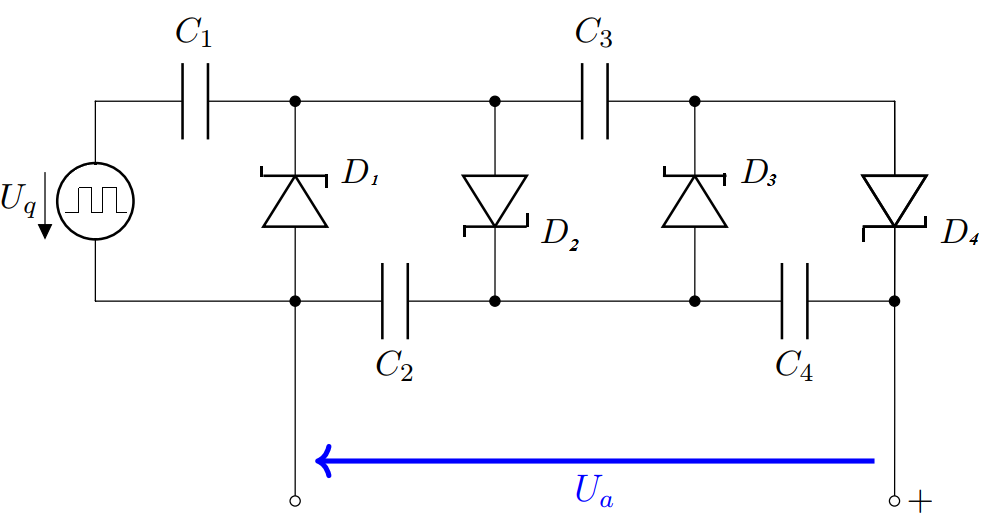
\includegraphics[width=0.8\textwidth]{schaltung}
	\captionof{figure}{4C/4D Kaskade als Vorlage zur Versuchsanordnung}
	\label{kaskadenschaltung}
\end{figure}


\laborsubsection{D}{Bilder können auch Nebeneinander}
\begin{figure}[H]
	\centering
	\begin{subfigure}[b]{0.45\textwidth} % b steht für am Boden ausrichten, damit beide captions auf gleicher Höhe
		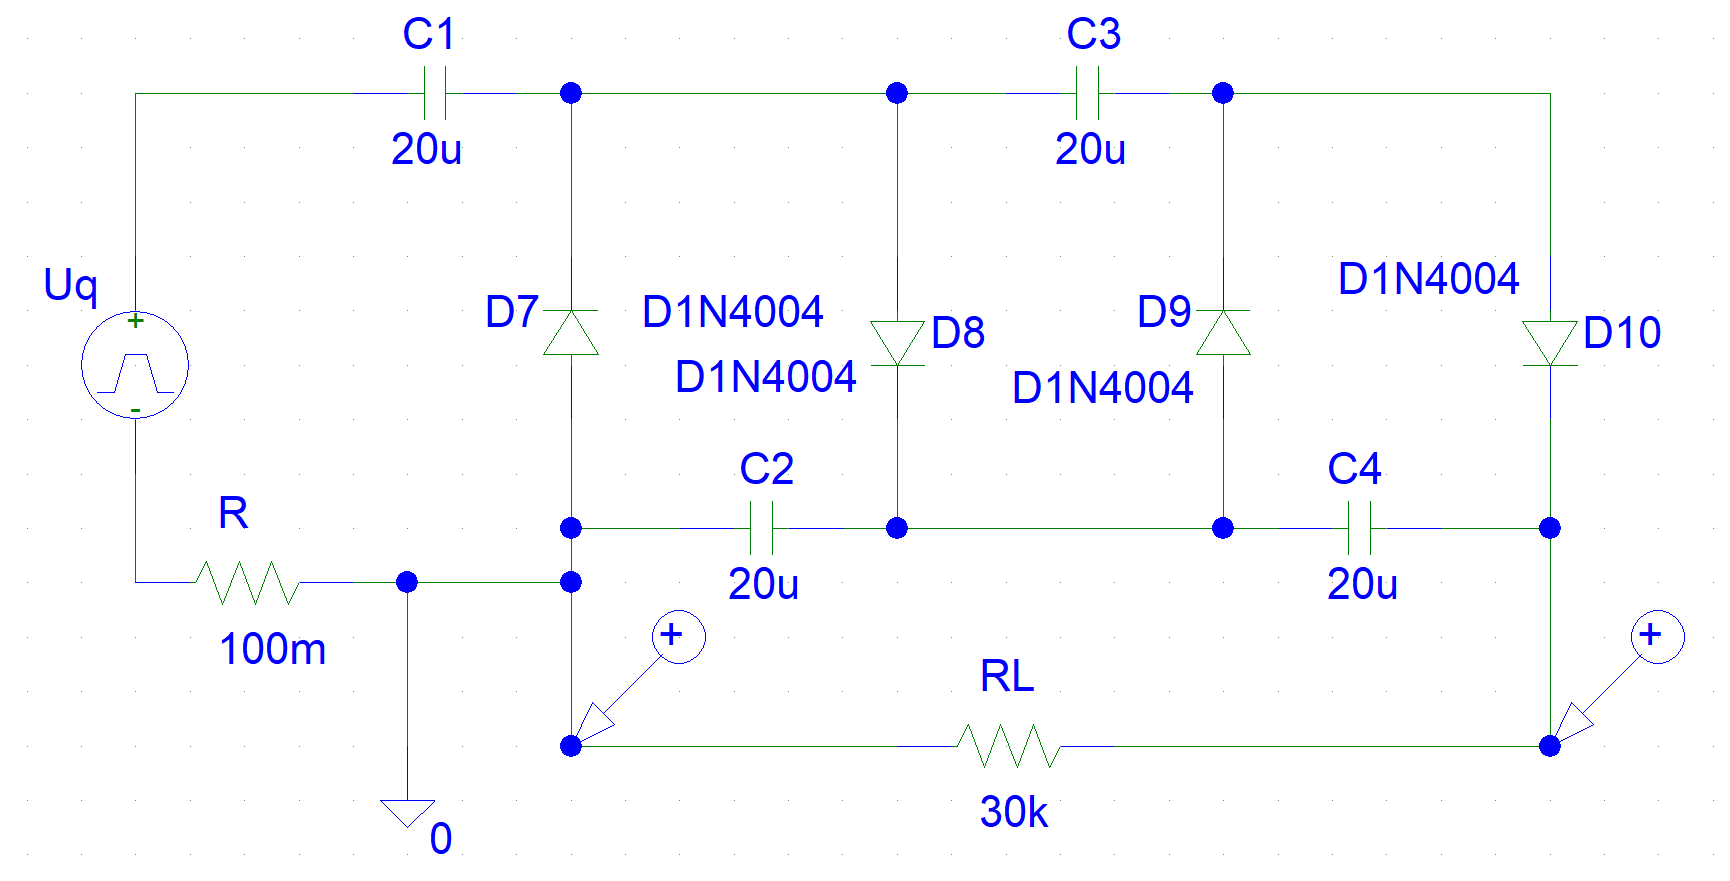
\includegraphics[width=\textwidth]{psch_kaskade}
		\subcaption{Simulation der Kaskadenschaltung (Marker für Spannungsmessung)}
		\label{psch_kaskade}
	\end{subfigure}
	\hfill % Um die beiden Figuren so weit wie möglich auseiannder zu machen
	% \hspace{0.1\textwidth} % Oder: Um einen festen Space zwischen den Figuren zu machen
	\begin{subfigure}[b]{0.45\textwidth}
		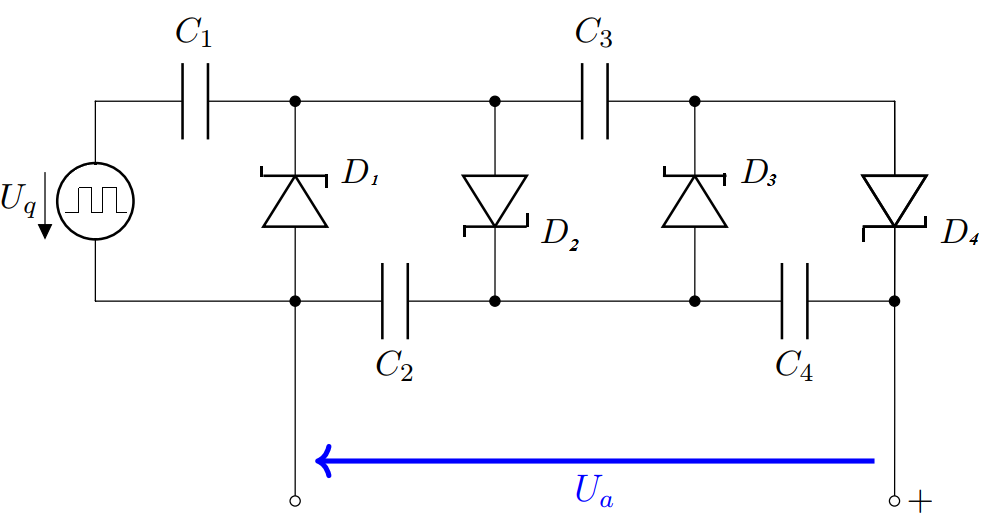
\includegraphics[width=\textwidth]{schaltung}
		\subcaption{4C/4D Kaskade als Vorlage zur Versuchsanordnung}
		\label{kaskadenschaltung_2}
	\end{subfigure}
	\caption{Gesamtdarstellung von irgendwas}
\end{figure}


\resetlaborsectioncounter
\laborsubsection{A}{Tabelle}

\begin{table}[H]
	\centering
	\renewcommand{\arraystretch}{2} % Senkrechten Abstand für diese Tabelle erhöhen
	\setlength{\tabcolsep}{0.3em} % Horizontalen Abstand für diese Tabelle erhöhen
	% S in table richtet diese nach kommata aus
	% dies funktioniert bei starkunsymetreischen zahlen nicht.
	% dazu kann man mit table-format = A.B die anzahl der erwarteten stellen eingeben dabei steht A für die Anzahl der zahlen vor dem komma und B fur die Anzahl hinter dem komma
	% test in der spalte mit {} umklammern bsp {text $P_A$}
	
	% \makecell{ 1. zeile \\ 2. zeile} ermögtlicht einfache zeilenumbrüche in einer zelle
	\begin{tabular}{|c|c|S[ table-format = 2.3]|S[ table-format = 2.3]|S[ table-format = 1.4]|S[ table-format = 1.4]|}
		\hline
		\multicolumn{2}{|c|}{}& {\makecell{Ergebnis\\ der Wirkleistung \\ aus der Simulation \\ in Watt}} & {\makecell{berechnete \\Wirkleistung\\ in Watt}} &{Abweichungen} &{\makecell{Abweichung\\ in \%}} \\ \hline
		\multirow{3}{*}{\makecell{$L_1$\\ als Bezug}} 
		&  $P_A$ & 15,500 & 15,4954 & 0,0046 & 0,0297 \\ \cline{2-6} 
		& $P_B$ & 47,761 & 47,7607 & 0,0003 & 0,0006 \\ \cline{2-6} 
		& $P_{ges}$ & 63,261 & 63,2561 & 0,0049 & 0,0077 \\ \hline
		\multirow{3}{*}{\makecell{$L_2$ \\als Bezug}}
		& $P_A$ & 38,398 & 38,3972 & 0,0008 & 0,0021 \\ \cline{2-6} 
		& $P_B$ & 24,863 & 24,8624 & 0,0006 & 0,0024 \\ \cline{2-6} 
		& $P_{ges}$ & 63,261 & 63,2596 & 0,0014 & 0,0022 \\ \hline
	\end{tabular}
\end{table}


\begin{table}[H]
	\centering
	\caption{The \texttt{s} column processes everything.}
	\label{tab:s:processing}
	\begin{tabular}{ss}
		\toprule
		{Unit} & \multicolumn{1}{c}{Unit}\\
		\midrule
		{\si{m^3}} & \multicolumn{1}{c}{\SI{}{m^3}} \\
		\kilogram & \kilogram \\
		\bottomrule
	\end{tabular}
\end{table}


